\documentclass{article}
\usepackage[UTF8]{ctex}
\usepackage{geometry}

\usepackage{listings}
\usepackage{float}
\usepackage{fancyhdr}
\usepackage{extramarks}
\usepackage{amsmath}
\usepackage{amsthm}
\usepackage{amsfonts}
\usepackage{tikz}
\usepackage{multicol}
\usepackage[ruled,vlined]{algorithm2e}
\usepackage{algpseudocode}
\usetikzlibrary{automata,positioning}

\geometry{left = 2cm, right = 2cm, top = 2cm, bottom = 2cm}

\author{黄道吉}
\title{ipv4协议收发实验报告}
\date{\today}

\begin{document}

\maketitle

IPv4协议是互联网的核心协议。这次实验要求实现IPv4协议中收发数据包的部分。这既包括实现IPv4协议向上一层协议提供的接口:接受来自高一层的数据包,按照IPv4进行封装,交给下一层;也包括实现本层基本的接受处理功能:接受本层的分组,检查其正确性,正确的转发给上层,否则报错丢弃。

\section{背景知识}

这次实验的中心是理解IPv4协议的报文组成,主要是报头的数据格式。我在实现的过程中主要参考了RFC791和RFC1071,前者定义了IPv4报文的结构,后者提供了计算header checksum的方法。下文会简要介绍本文用到的部分。

\subsection{IPv4报头格式}

下图描述了IPv4报头的格式。本次实验关心的是以下部分
\begin{itemize}
    \item version: 对于IPv4,version = 4
    \item IHL: 是指报头长度,以word(32 bits)为单位。对于一个有效的报头,IHL最小为5,最长的报头只有15个words(RFC791在total length处提到),本次实验并不考虑option部分,所以发送报文时报头长度为5。
    \item total length: 整个报文的长度,以Byte(8 bits)为单位,包含报头和数据。
    \item TTL: 报文剩余存货的时间。如果这个域为0,接受时应当丢弃。
    \item header checksum: 只对报头部分计算checksum,计算方法在下面有介绍。
    \item source/destination address: 发送和接受地址。如果接收地址为本机地址或广播地址,则应接受。

\end{itemize}

\begin{figure}[H]
    \centering
    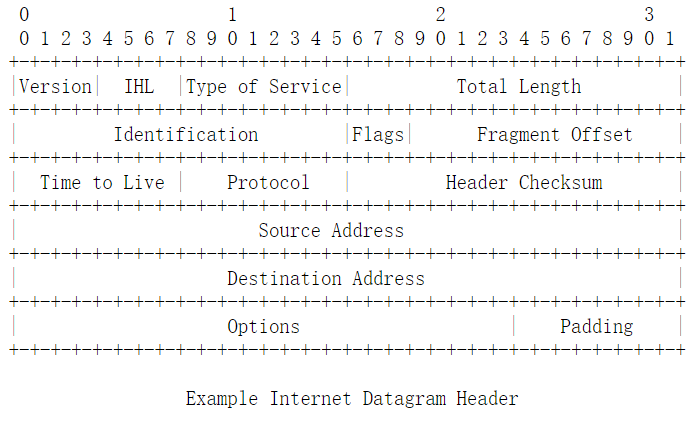
\includegraphics[width=0.7\textwidth]{header.png}
    \caption{ipv4 header, fig from RFC791}
    \label{1}
\end{figure}

\subsection{checksum算法}

internet checksum算法在RFC1071中有定义和参考的实现。我在实现过程中参考了这一部分的内容。checksum算法将报头按16bits一组分开,分别相加,并将结果的进位部分加到最低位,取反的结果填充到报头中的checksum部分。这样填充好的报头再次进行checksum操作的时候应当结果为0。在进行checksum时有几个地方是需要注意的
\begin{itemize}
    \item 初始时checksum部分应当为0
    \item 计算checksum和填充checksum时,因为牵扯到两个字节一组,对于组内字节的顺序应使用同一种大小端字节序,采用哪一个字节序对结果没有影响。我的实现使用大端字节序,即报文的第一个16bits在计算时看作 $version \times 2^{12} + IHL \times 2^{8} + type\ of\ service$,并且checksum的高位存储在报头的10字节(从0计数),低位在11字节。
    \item 将进位加到最低位的过程可能需要不止一次,例如checksum中间结果为0x0001FFFF时,应当进行两次操作。
\end{itemize}

\section{实现细节}

本节介绍我的实现的细节和只参考手册和查阅资料没有解决的问题。

\subsection{接受报文}

检查报文合法性阶段需要分别检验上文提到的各个域,其间的变量最好全部取成无符号整数,以便移位操作不需要考虑符号的问题。在检查目的地址时,如果目的地址是本机地址则必须接受,但广播地址并没有很好的定义,除了255.255.255.255以外,回环地址127.0.0.0/8和链路本地地址169.254.0.0/16是否也需要考虑进去。这可能需要在线上调试的过程中检查。RFC中定义的checksum的过程有考虑字节数为奇或偶的情况,我们的设定中报头都是以word为最小长度单位的,不存在奇字节的情况。

\subsection{发送报文}

发送报文时,因为这次试验不考虑option域,报头长度为5。因为不清楚编译代码的机器是大端还是小端序,因此保险起见按字节填充报头的各个域。


\section{代码实现}


\lstset{language=C++,
%backgroundcolor=\color{write},
basicstyle=\footnotesize,
keywordstyle=\color{blue}\bfseries,
commentstyle=\color{gray},
}

\lstset{breaklines}
\lstset{extendedchars=false}

\begin{lstlisting}
#include <memory.h>

/* API provided by system */

void ip_DiscardPkt(char * pBuffer ,int type);
void ip_SendtoLower(char *pBuffer ,int length);
void ip_SendtoUp(char *pBuffer, int length);
unsigned int getIpv4Address();

int stud_ip_recv(char * pBuffer, unsigned short length){

    // in case version == 1xxx, which would also yield VERSION_ERROR, but just to be concise
    unsigned int version = ((unsigned int)pBuffer[0]) >> 4;
    if(version != 4){
        ip_DiscardPkt(pBuffer, STUD_IP_TEST_VERSION_ERROR);
        return -1;
    }

    unsigned int ip_head_length = ((unsigned int)pBuffer[0]) & 0xF;
    if(ip_head_length < 5 || ip_head_length > 15){
        // according to RFC791, ip_head_length <= 15
        // see RFC791 section 3.1, mentioned in "total length" part
        // ref: https://tools.ietf.org/html/rfc791
        ip_DiscardPkt(pBuffer, STUD_IP_TEST_HEADLEN_ERROR);
        return -1;
    }

    unsigned int time_to_live = ((unsigned int)pBuffer[8]);
    if(time_to_live == 0){
        ip_DiscardPkt(pBuffer, STUD_IP_TEST_TTL_ERROR);
        return -1;
    }

    unsigned int destination_address = ntohl(*(unsigned int* )(pBuffer + 16)); // might be wrong
    if(destination_address != getIpv4Address() || destination_address != (~0)){
        // if it is necessray to consider
        //     - localhost address: 127.0.0.0/8
        //     - link-local address: 169.254.0.0/16
        // then check: (dst_addr >> 24) != 127 and (dst_addr >> 16) != ((169 << 8) + 254)
        ip_DiscardPkt(pBuffer, STUD_IP_TEST_DESTINATION_ERROR);
        return -1;
    }

    unsigned int header_checksum = 0;
    for(int i = 0; i < 4 * ip_head_length; i += 2){
        // 4 * IHL % 2 == 0, no need to consider odd/even issue
        header_checksum += (pBuffer[i] << 8) + pBuffer[i + 1];
    }
    while(header_checksum >> 16){
        // in case header_checksum == 0x1FFFF
        // add once might not be enough
        // ref: https://tools.ietf.org/html/rfc1071 section 4.1

        // we stick to big-endian byte order, since checksum is byte order independent
        // ref: https://tools.ietf.org/html/rfc1071 section 1.2.(B)
        header_checksum == (header_checksum >> 16) + (header_checksum & 0xFFFF);
    }
    header_checksum = ~header_checksum;

    if(header_checksum != 0){
        ip_DiscardPkt(pBuffer, STUD_IP_TEST_CHECKSUM_ERROR);
        return -1;
    }

    ip_SendtoUp(pBuffer, length);

    return 0;
}

int stud_ip_Upsend(char* pBuffer, unsigned short len, unsigned int srcAddr,
    unsigned int dstAddr ,byte protocol, byte ttl){

    unsigned int version = 4;
    unsigned int ip_head_length = 5; // no option header in this case
    unsigned int total_length = 4 * ip_head_length + len;


    unsigned char* total_buffer = malloc(total_length);
    memset(total_buffer, 0, total_length);

    total_buffer[0] = (version << 4) | ip_head_length;
    // type of service not specified -> set to zero
    total_buffer[2] = total_length >> 8;
    total_buffer[3] = total_length & 0xFF;
    // identification, flags, fragment offset not specified
    total_buffer[8] = time_to_live;
    total_buffer[9] = protocol;

    total_buffer[12] = srcAddr >> 24;
    total_buffer[13] = srcAddr >> 16;
    total_buffer[14] = srcAddr >> 8;
    total_buffer[15] = srcAddr & 0xFF;

    total_buffer[16] = dstAddr >> 24;
    total_buffer[17] = dstAddr >> 16;
    total_buffer[18] = dstAddr >> 8;
    total_buffer[19] = dstAddr & 0xFF;

    unsigned int header_checksum = 0;
    for(int i = 0; i < 20; i += 2){
        header_checksum += (total_buffer[i] << 8) + total_buffer[i + 1];
    }
    while(header_checksum >> 16){
        header_checksum == (header_checksum >> 16) + (header_checksum & 0xFFFF);
    }
    header_checksum = ~header_checksum;
    total_buffer[10] = header_checksum >> 8;
    total_buffer[11] = header_checksum & 0xFF;

    memcpy(total_buffer + 20, pBuffer, len);

    ip_SendtoLower(total_buffer, total_length);

    return 0;
}

\end{lstlisting}


\end{document}
